\slide{Aquisição}{

\begin{itemize}
    \item Doutorando Fábio e DETRAN
    \item Avenida Hélio Prates
    \item Registro de veículos de Maio a Junho de 2016
\end{itemize}

}

\slide{Características do Tráfego}{
    O tráfego é afetado por diversos fatores.

    \begin{itemize}
        \item \textbf{Fatores Temporais}. Ex: Alto fluxo causado pelo horário do expediente dos trabalhadores;
        \item \textbf{Fatores Espaciais}. Ex: Locais que podem ter mais ou menos movimento de veículos (áreas rurais, urbanas, próximas de empresas, etc);
        \item \textbf{Fatores Aleatórios}. Ex: Eventos impossíveis de prever que podem afetar o fluxo de veículos, como acidentes automobilísticos.
    \end{itemize}
    
    % should we talk here that we are only gonna use temporal and spatial features or we just talk about it?
}

%colocar referncia do artigo que demonstra como se calcula a densidade : Short-Term Traffic Prediction Using Long Short-Term Memory Neural Networks Zainab Abbas et al
\slide{Interpretação do Tráfego}{
    \begin{itemize}
        \item \textbf{Fluxo}: Quantidade de veículos em um determinado intervalo de tempo;
        \item \textbf{Velocidade Média}: Velocidade média dos veículos nesse mesmo intervalo de tempo;
        \item \textbf{Densidade}: Velocidade média dos veículos em um intervalo de tempo multiplicado pelo fluxo de veículos neste mesmo intervalo.
    \end{itemize}
}

\slide{Caracterização dos Dados}{
    \begin{itemize}
        \item Os registros disponibilizados estão organizados em 8 colunas e foram coletados por um total de 8 sensores. Com exceção da coluna \textit{ID.Equip}, todas as colunas são quantitativas.
    \end{itemize}
}

\slide{Caracterização dos Dados}{
    \begin{table}[htbp]
        \begin{tabular}{ccccccc}
        \toprule
        \multicolumn{1}{l}{\textbf{Id Equi.}} & \multicolumn{1}{l}{\textbf{A/M/D}} & \multicolumn{1}{l}{\textbf{Hora}} & \multicolumn{1}{l}{\textbf{Faixa}} & \multicolumn{1}{l}{\textbf{km/h}} & \multicolumn{1}{l}{\textbf{km/h Max}} & \multicolumn{1}{l}{\textbf{Tam.}} \\ 
        \midrule
        RSI128 & 2016/5/1 & 00:00:09 & 1 & 20 & 60 & 0 \\
        RSI131 & 2016/5/1 & 00:00:09 & 2 & 45 & 60 & 1.1 \\
        RSI132 & 2016/5/1 & 00:00:09 & 1 & 40 & 60 & 0 \\
        RSI131 & 2016/5/1 & 00:00:10 & 1 & 35 & 60 & 0.5 \\ 
        \bottomrule
        \end{tabular}
        \label{table:data}
        \caption{Exemplo dos dados coletados pelo DETRAN}
    \end{table}
}

\slide{Escopo dos Dados}{
    \begin{itemize}
        \item Os registros dizem respeito a apenas 3 meses de dados coletados especificamente em Taguatinga, Brasília. Logo, a metodologia utilizada pode não servir para outros meses, ou localidades.
        \item Existem também cenários em que os fiscalizadores não conseguem registrar corretamente, como :
        \begin{itemize}
            \item Falhas no equipamento;
            \item Bloqueio nas vias;
            \item Acidentes de trânsito;
            \item Greves, eventos, etc.
        \end{itemize}
    \end{itemize}
}

\slide{Cruzamento 1}{
    \begin{figure}[htbp]
        \centering
        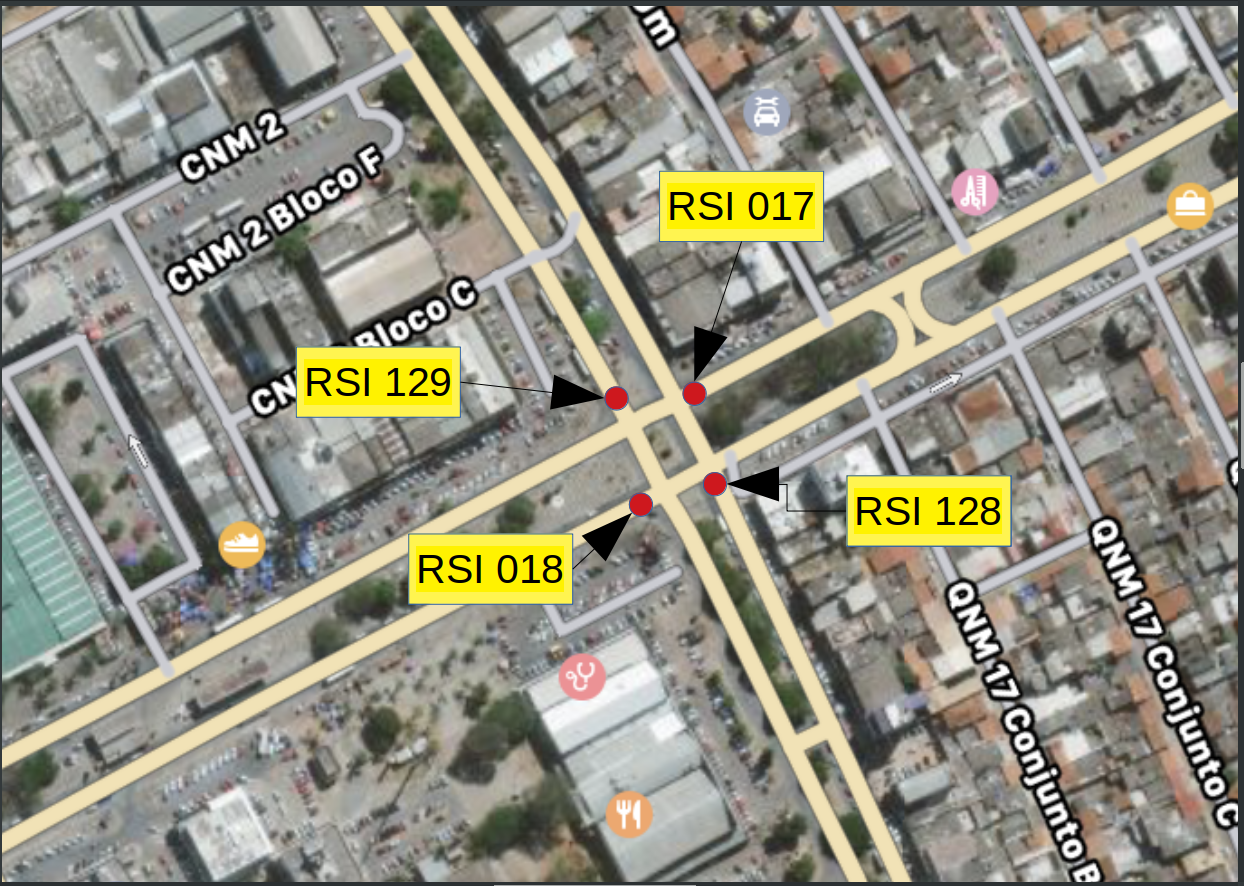
\includegraphics[scale=0.2]{monography/img/maps/crossing_1.png}
    \end{figure}
}

\slide{Cruzamento 2}{
    \begin{figure}[htbp]
        \centering
        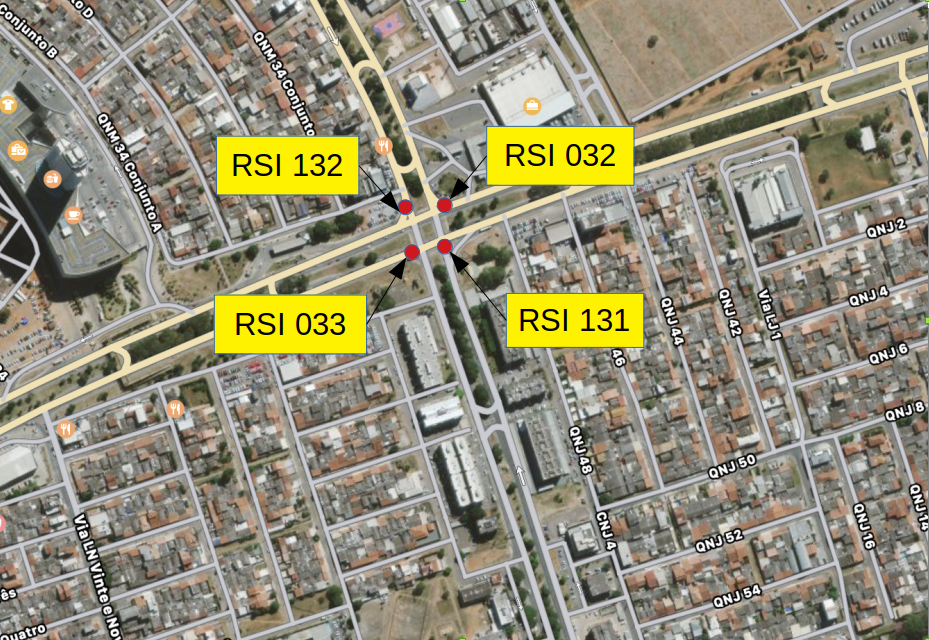
\includegraphics[scale=0.3]{monography/img/maps/crossing_2.png}
    \end{figure}
}
